\documentclass[11pt,class=report,crop=false]{standalone}
\usepackage[screen]{../python}


\begin{document}


%====================================================================
\chapitre{Automates}
%====================================================================

\index{automate}

\objectifs{Tu vas programmer des automates cellulaires qui, à partir de règles simples, produisent des visualisations amusantes.}

\begin{center}
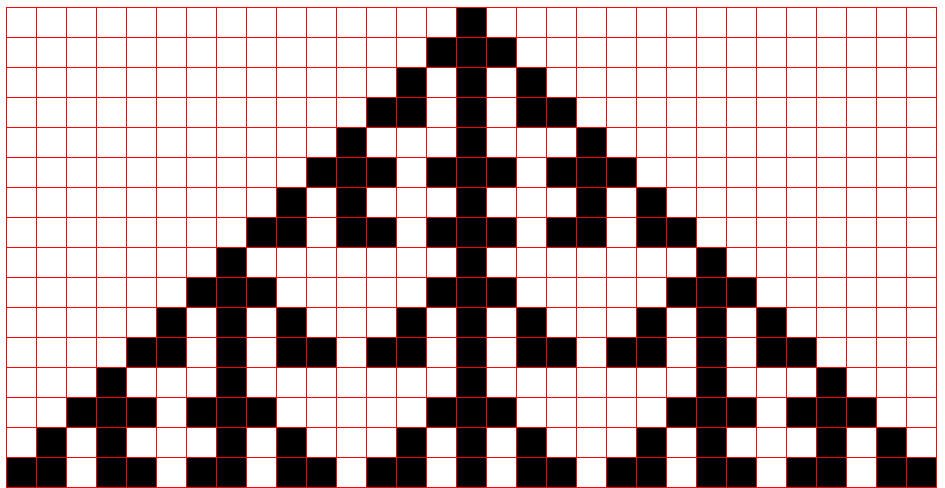
\includegraphics[scale=\myscale,scale=0.25]{ecran-automate-0}
\end{center}	

%%%%%%%%%%%%%%%%%%%%%%%%%%%%%%%%%%%%%%%%%%%%%%%%%%%%%%%%%%%%%%%%
%%%%%%%%%%%%%%%%%%%%%%%%%%%%%%%%%%%%%%%%%%%%%%%%%%%%%%%%%%%%%%%%


%%%%%%%%%%%%%%%%%%%%%%%%%%%%%%%%%%%%%%%%%%%%%%%%%%%%%%%%%%%%%%%%
% Activité 1
%%%%%%%%%%%%%%%%%%%%%%%%%%%%%%%%%%%%%%%%%%%%%%%%%%%%%%%%%%%%%%%%


\begin{activite}[Une suite logique]

\objectifs{Objectifs : programmer une suite logique amusante (mais pas nécessaire pour l'activité suivante).}

Voici une suite :
\begin{center}
1 \\
11 \\
21 \\
1211 \\
111221 \\
312211 \\
13112221 \\
1113213211
\end{center}

Pour passer d'une ligne à la suivante, il suffit de lire à haute voix en comptant les nombres !
Par exemple la ligne 1211 est lue \og{}un un (pour 1), un deux (pour 2), deux un (pour 1 1)\fg{}, la ligne d'après est donc 111221 !
Cette dernière ligne se lit \og{}trois uns, deux deux, un un\fg{} donc la ligne suivante sera 312211.


Programme une fonction \ci{lecture(mot)} qui calcule et renvoie la lecture de la chaîne \ci{mot}.
Par exemple \ci{lecture("1211")} renvoie \ci{"111221"}.


\begin{itemize}
  \item Essaie de programmer cette fonction sans lire les indications suivantes !

  \item \emph{Indications.}
Tu peux utiliser trois variables : une variable qui lit chaque caractère du mot, une variable correspondant au caractère précédent, un compteur à incrémenter si ces deux caractères sont égaux.
  
  \item \emph{Algorithme.} 
  Si tu n'y arrives pas tout seul, voici les grandes lignes d'un algorithme possible.

Pour chaque caractère du mot :
\begin{itemize}
  \item si le caractère est le même que le caractère précédent, incrémenter le compteur,
  \item sinon, rajouter au mot à créer la valeur du compteur suivie du caractère précédent.
\end{itemize}
À la fin, il faut aussi rajouter au mot à créer la valeur du compteur suivie du caractère précédent.
\end{itemize}

\smallskip

\emph{Question.} Trouve le premier mot qui contient \ci{33}. 
\end{activite}


%%%%%%%%%%%%%%%%%%%%%%%%%%%%%%%%%%%%%%%%%%%%%%%%%%%%%%%%%%%%%%%%
%%%%%%%%%%%%%%%%%%%%%%%%%%%%%%%%%%%%%%%%%%%%%%%%%%%%%%%%%%%%%%%%

\begin{cours}[Automates linéaires]

On travaille sur des lignes superposées, formées de cases.
Chaque case peut contenir une cellule (la case est alors noire/contient $1$) ou être vide (la case est blanche/contient $0$).

\myfigure{0.7}{
\tikzinput{fig-automate-1}
}


Un \defi{automate linéaire} est une règle qui à partir du contenu de trois cases consécutives sur une ligne, détermine le contenu de la case sur la ligne du dessous.

La \defi{règle} est donc donnée par la liste des $8$ configurations possibles au départ, avec pour chacune la naissance ou pas d'une cellule en-dessous.

\myfigure{0.7}{
\tikzinput{fig-automate-2}
}




\textbf{Exemple.}
\begin{itemize}
  \item Partons d'une seule cellule qui sera sur la ligne du haut.
 
\myfigure{0.6}{
\tikzinput{fig-automate-8a}
}   
  
  
  \item Et choisissons la règle définie par les configurations : \\
  
\myfigure{0.7}{
\tikzinput{fig-automate-7}
}   
    
   \item Pour décider de la naissance d'une cellule dans une case de la ligne en-dessous, on regarde les trois cases au-dessus et on applique la règle. Sur le dessin
 ci-dessous deux cellules sont vivantes après l'évolution (on a indiqué par des flèches seulement les règles pour lesquelles une cellule apparaît). \\
   
\myfigure{0.6}{
\tikzinput{fig-automate-8b}
}   

 \item On peut itérer le processus. Une seule cellule apparaît lors de cette seconde évolution.
 
\myfigure{0.6}{
\tikzinput{fig-automate-8c}
}   

      
\end{itemize}
 
\textbf{Notations.}

\begin{itemize}
  \item On note $0$ pour une case vide et $1$ pour une case contenant une cellule vivante.

  \item Un ligne est représentée par une liste de $0$ et de $1$. Par exemple 
  \ci{[0,0,0,1,0,1,0,1,0,0]} est une ligne de $10$ cases, contenant $3$ cellules.
  
  \item La règle est codée par une liste de $0$ et $1$ et de longueur $8$, déterminée par l'image des $8$ configurations possibles. Par exemple : 
 $[0,0,1,0,1,1,0,1]$ correspond à la règle :
 
 \smallskip
 
\myfigure{0.7}{
\tikzinput{fig-automate-3}
} 

  
\end{itemize}
 
\end{cours}

%%%%%%%%%%%%%%%%%%%%%%%%%%%%%%%%%%%%%%%%%%%%%%%%%%%%%%%%%%%%%%%%
% Activité 2
%%%%%%%%%%%%%%%%%%%%%%%%%%%%%%%%%%%%%%%%%%%%%%%%%%%%%%%%%%%%%%%%


\begin{activite}[Automates linéaires]

\objectifs{Objectifs : calculer et afficher les automates linéaires.}

\begin{center}
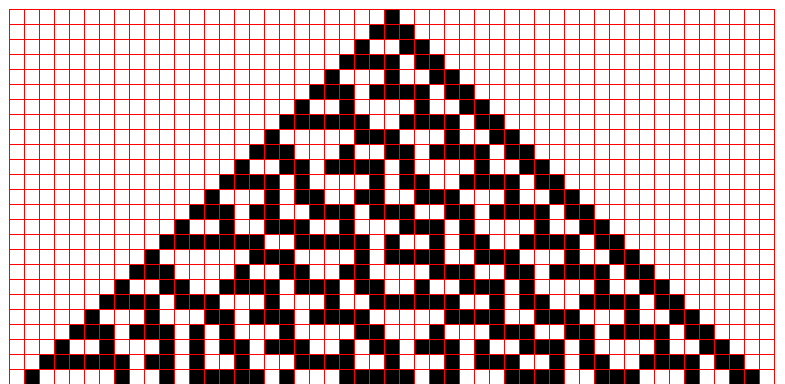
\includegraphics[scale=\myscale,scale=0.4]{ecran-automate-6}
\end{center}	

\begin{enumerate}
  \item \textbf{Évolution d'une cellule.} Programme une fonction \ci{cellule_suivante(a,b,c,regle)}
  qui calcule et renvoie la couleur (0 ou 1) de la case
  située sous les trois cases contenant \ci{a}, \ci{b}, \ci{c} selon la règle
  donnée.
  
  \myfigure{0.7}{
\tikzinput{fig-automate-4}
} 
  
  \begin{itemize}
    \item \ci{a}, \ci{b}, \ci{c} sont les couleurs ($0$ ou $1$) des cases situées au-dessus ($a$ est la case la plus à gauche).
    \item La loi de transformation est donnée par la liste \ci{regle} formée d'une suite de $8$ entiers $0$ ou $1$. 
    
    \item Exemple avec \ci{regle = [0,0,1,0,1,1,0,1]} alors \ci{cellule_suivante(0,0,0, regle)} renvoie \ci{0}, 
    \ci{cellule_suivante(0,0,1, regle)} renvoie aussi \ci{0},  \ci{cellule_suivante(0,1,0, regle)} renvoie \ci{1}, etc.
    
  \item Si tu ne veux pas écrire les $8$ cas possibles, calcule $4a+2b+c$ ! 
  \end{itemize}
  
  \item \textbf{Affichage de la règle.} Déduis-en une fonction \ci{affiche_regle(regle)} qui affiche à l'écran la règle donnée sous la forme \og{}$a,b,c \rightarrow d$\fg{} où $d$ est la couleur de la nouvelle case, par exemple :
\begin{lstlisting}
0 0 0  ->  0
0 0 1  ->  0
0 1 0  ->  1
...
\end{lstlisting}

	\item \textbf{Évolution d'une ligne.} Programme une fonction \ci{ligne_suivante(ligne,regle)}
	qui à partir d'une liste \ci{ligne} formée de $0$ et $1$, calcule
	les cellules de la ligne suivante (renvoyée sous la forme d'une liste de $0$ et de $1$). 
	
	\emph{Exemple.} Avec la règle $[0,0,1,0,1,1,0,1]$ alors la ligne suivant $[0, 0, 1, 0, 1]$ est la ligne $[0, 0, 1, 1, 1]$.
	
  \myfigure{0.7}{
\tikzinput{fig-automate-5}
} 	
	
	\emph{Remarque.} Lors du calcul des cases situées à l'une des deux extrémités de la ligne, on considère qu'au delà, il n'y a pas de cellule (c'est donc comme si à droite et à gauche de la ligne initiale il y avait un $0$).

  \myfigure{0.7}{
\tikzinput{fig-automate-6}
} 		
	
  \item 	\textbf{Itérations.} Déduis-en une fonction \ci{plusieurs_lignes(n,ligne,regle)} qui affiche sur le terminal les $n$ lignes qui suivent la ligne donnée. 
	
\emph{Exemple.}
Toujours avec la règle $[0,0,1,0,1,1,0,1]$,
pars d'une ligne définie par une seule cellule au milieu :
\mycenterline{\ci{ligne = [0]*10 + [1] + [0]*10}}
Alors l'itération du processus correspond à l'évolution d'une cellule,
qui voyage vers la droite en se dédoublant une fois sur deux.

\begin{center}
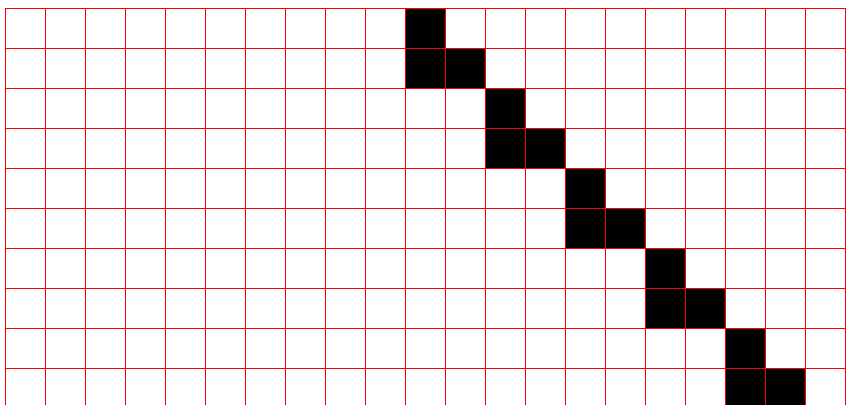
\includegraphics[scale=\myscale,scale=0.3]{ecran-automate-8}
\end{center}

  \item \textbf{Affichage.} Programme une fonction \ci{afficher_lignes(n,ligne,regle)} qui réalise un bel affichage graphique d'une ligne de cellules et de son évolution sur $n$ lignes.
La présence d'une cellule (marquée par $1$) est affichée par une case noire, l'absence de cellule (marquée par $0$) est affichée par une case blanche. 

\begin{center}
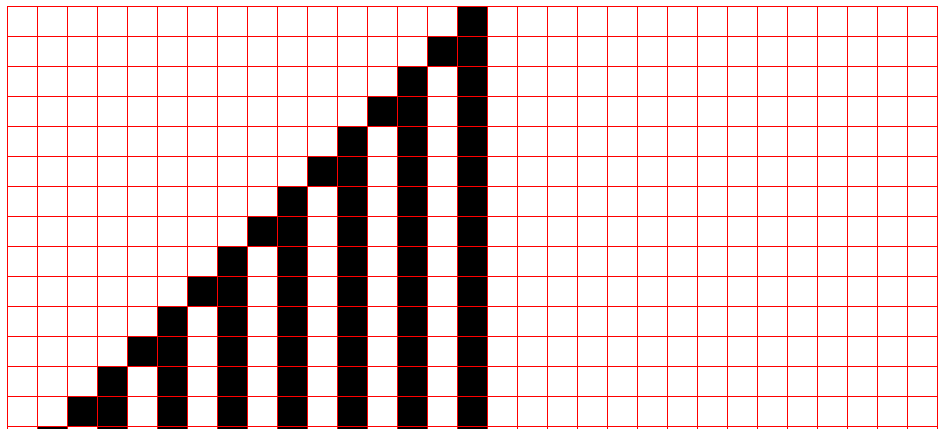
\includegraphics[scale=\myscale,scale=0.3]{ecran-automate-7}
\end{center}
  
  
  \item \textbf{Numérotation des règles.}
  Il y a en tout $2^8 = 256$ règles possibles, car une règle est une liste de $8$ \emph{bits}.
  On décide donc de numéroter la règle en fonction du nombre binaire représenté par la liste :
  
  $$\underbrace{[0,0,1,0,1,1,0,1]}_{\text{règle}} 
  \qquad \longleftrightarrow \qquad
  \underbrace{0.0.1.0.1.1.0.1}_{\text{nombre binaire}}
  \qquad \longleftrightarrow \qquad  
  \underbrace{45}_{\text{numéro}}  
  $$
  
	
	Écris une fonction \ci{definir_regle(numero)} qui n'est autre que la conversion d'un entier en écriture binaire sur $8$ \emph{bits}.
	Par exemple \ci{definir_regle(45)} renvoie la règle $[0,0,1,0,1,1,0,1]$.


\begin{algorithme}
  \sauteligne 
 \begin{itemize}
   \item
   \begin{itemize}
     \item Entrée : un entier $n$ entre $0$ et $255$.
     \item Sortie : le nombre $n$ en écriture binaire sous la forme d'une liste de $8$ \emph{bits}.
   \end{itemize}

  \item Démarrer avec une liste vide.
  
  \item Répéter $8$ fois :
   \begin{itemize}
     \item Ajouter $n \, \% \, 2$ au début de la liste.
     \item Faire $n \leftarrow n \, // \, 2$.
   \end{itemize}
   
   \item Renvoyer la liste.
   
 \end{itemize}  
 \end{algorithme}

	
% \emph{Remarque.} La convention de numérotation choisie ici n'est pas celle définie habituellement.
	
	
  \item \textbf{Types d'automates.}
  
  En partant d'une seule cellule, essaie de trouver différents types de comportements :
  \begin{itemize}
    \item des automates cellulaires qui convergent vers un état stable (voire vide),
    \item des automates cellulaires qui convergent vers un état périodique,
    \item des automates cellulaires ayant des structures symétriques (par exemple, qui réalisent des triangles de Sierpinski),
    \item des automates cellulaires avec des structures qui semblent aléatoires.
  \end{itemize}
  	


\begin{center}
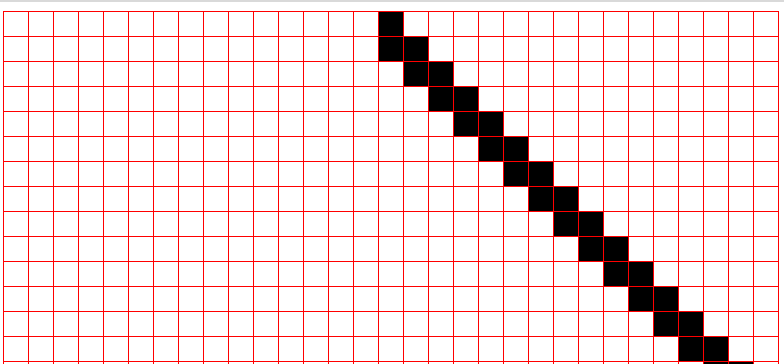
\includegraphics[scale=\myscale,scale=0.2]{ecran-automate-3}
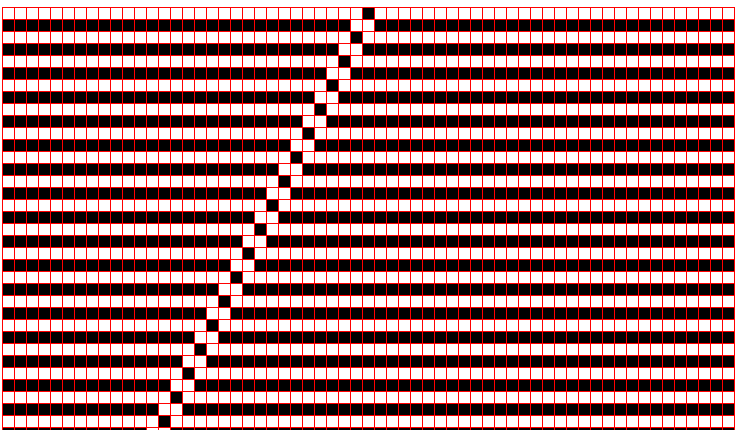
\includegraphics[scale=\myscale,scale=0.2]{ecran-automate-2}
\end{center}	

\begin{center}
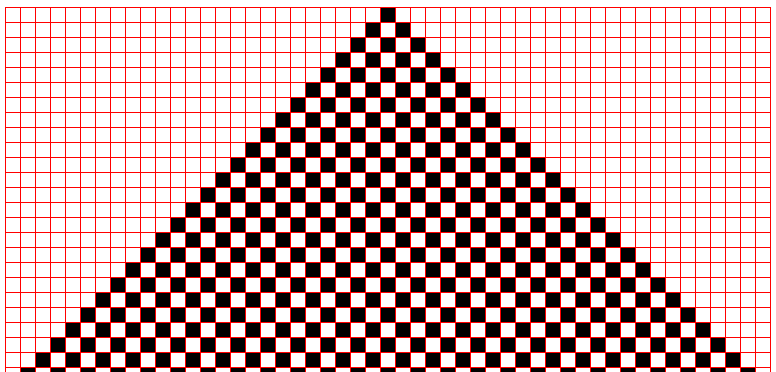
\includegraphics[scale=\myscale,scale=0.2]{ecran-automate-4}
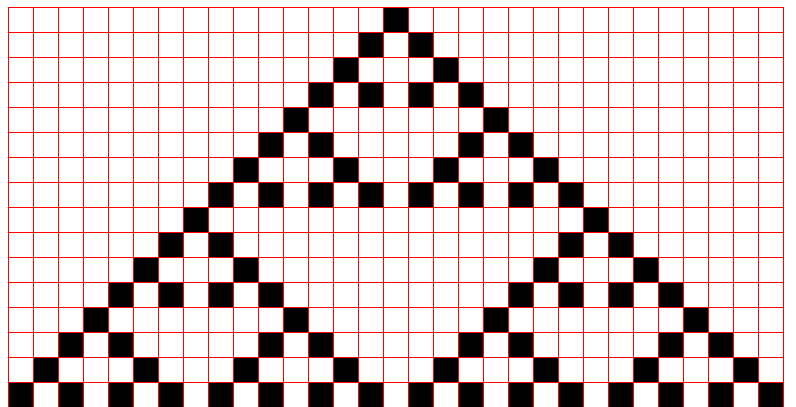
\includegraphics[scale=\myscale,scale=0.2]{ecran-automate-5}
\end{center}	

\begin{center}
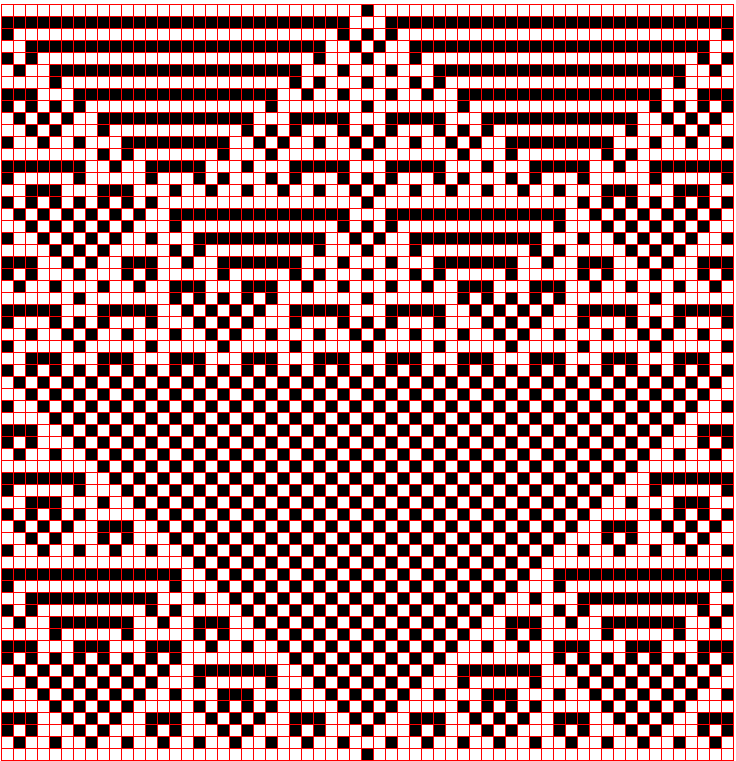
\includegraphics[scale=\myscale,scale=0.2]{ecran-automate-1}
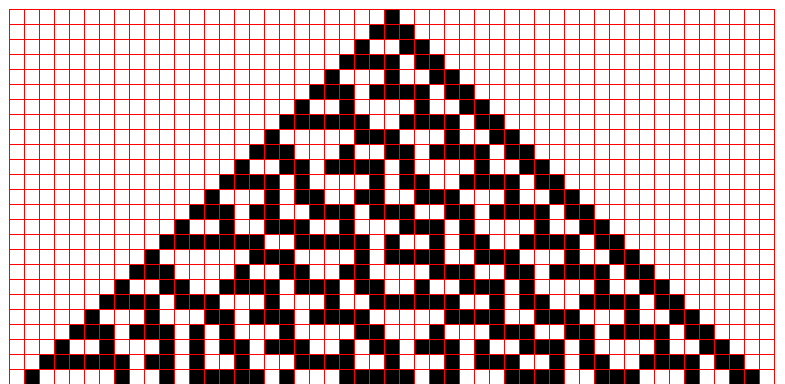
\includegraphics[scale=\myscale,scale=0.2]{ecran-automate-6}
\end{center}	




\end{enumerate}



\end{activite}

%%%%%%%%%%%%%%%%%%%%%%%%%%%%%%%%%%%%%%%%%%%%%%%%%%%%%%%%%%%%%%%%
%%%%%%%%%%%%%%%%%%%%%%%%%%%%%%%%%%%%%%%%%%%%%%%%%%%%%%%%%%%%%%%%

\end{document}
